\documentclass[]{article}
\usepackage{mathtools}
\usepackage[pdftex]{graphicx}	
\usepackage{amsmath,amsfonts,amsthm}	
\usepackage{tikz}
\usetikzlibrary{chains, positioning}
\newtheorem{theorem}{Theorem}[section]
\newtheorem{lemma}[theorem]{Lemma}
\newtheorem{proposition}[theorem]{Proposition}
\newtheorem{corollary}[theorem]{Corollary}

\theoremstyle{definition}
\newtheorem{definition}{Definition}[section]

\usetikzlibrary{calc,arrows}

%opening
\title{Neural network is universal approximator, why sigmoids?}
\author{Rafa\"l Skrzypiec}
\date{}
\begin{document}
\maketitle

\begin{center}
	
	
	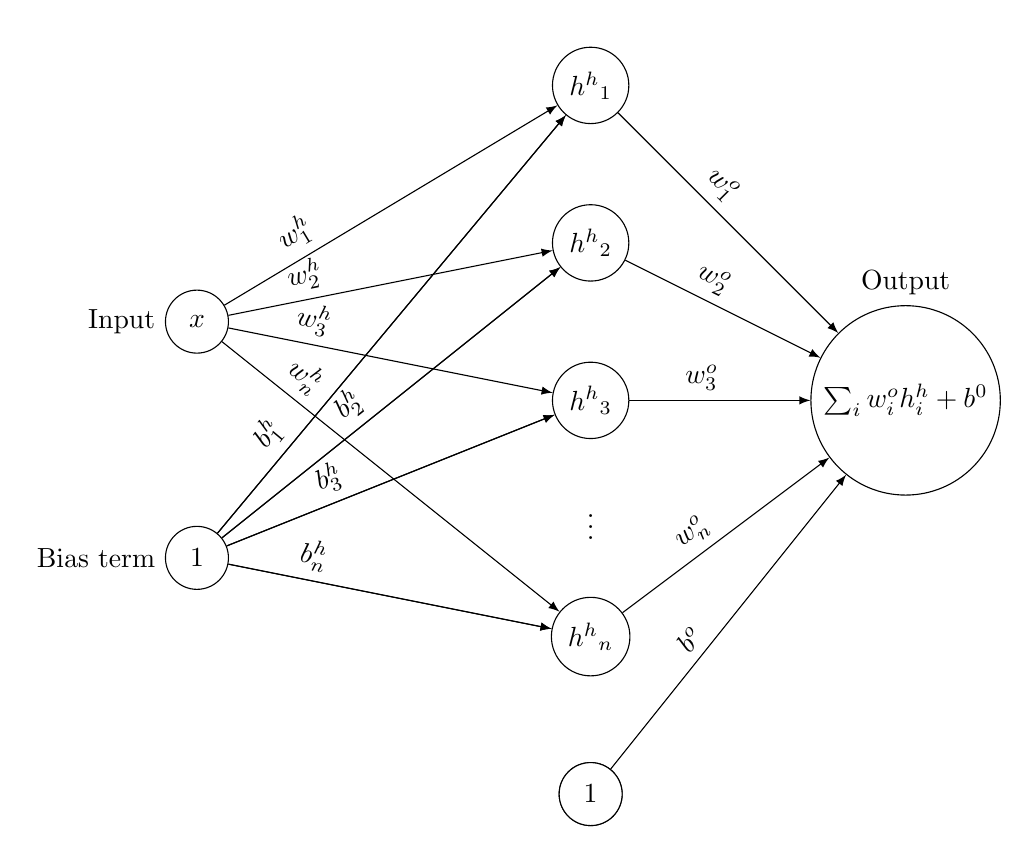
\begin{tikzpicture}
	[   cnode/.style={draw=black,draw=black,fill=#1,minimum width=8mm,circle},
	]
	\tikzset{normal arrow/.style={draw,-latex}}
	\node[cnode=white,label=90:Output] (s) at (9,-6) {$\sum_{i} w^o_{i} h^h_i + b^0$};
	\node[cnode=white,label=180:Bias term] (x-2) at (0,-8) {1};
	\node[cnode=white,label=180:] (p-5) at (5,-11) {1};
	\node at (5,-7.5) {$\vdots$};
	
	\node[cnode=white,label=180:Input] (x-1) at (0,-5) {$x$};
	
	\foreach \x in {1,...,5}
	{
		\pgfmathparse{\x<4 ? \x : "n"}	   
		\ifnum \x = 4
		
		
		\node[cnode=white,label=90:] (p-\x) at (5,{-2.*\x-div(\x,4)}) {${h^h}_n$};
		
		\else
		
		\ifnum \x = 5
		
		
		\node[cnode=white,label=90:] (p-\x) at (5,{-2*\x-div(\x,4)}) {$ 1 $};
		
		\else
		
		\node[cnode=white,label=90:] (p-\x) at (5,{-2*\x-div(\x,4)}) {${h^h}_{\x}$};
		
		\fi
		
		
		\fi
		\ifnum \x = 5
		\path[normal arrow] (p-\x) -- node[above,sloped,pos=0.4] {$b^{o}$} (s);
		\else
		\path[normal arrow] (p-\x) -- node[above,sloped,pos=0.4] {$w^o_{\pgfmathresult}$} (s);
		\fi
	}
	
	
	\foreach \x in {1,...,2}
	{   
		\foreach \y in {1,...,4}
		{   
			\ifnum \x=1
			\ifnum \y=4
			\path[normal arrow] (x-\x) -- (p-\y) node[above,sloped,pos=0.2] {$w^h_{n}$};
			
			\else
			\ifnum \y=5
			\path[normal arrow] (x-\x) -- (p-\y) node[below,sloped,pos=0.15] {$w_{w n+1}$};
			\else 
			\path[normal arrow] (x-\x) -- (p-\y) node[above,sloped,pos=0.25] {$w^h_{\y}$};
			
			\fi
			\fi
			\else
			\path[normal arrow] (x-\x) -- (p-\y); 		
			\fi
			
			\ifnum \x=2
				\ifnum \y=4
				\path[normal arrow] (x-\x) -- (p-\y) node[above,sloped,pos=0.25] {$b^h_{n}$};
					\else
				\ifnum \y=2
				\path[normal arrow] (x-\x) -- (p-\y) node[above,sloped,pos=0.42] {$b^h_{\y}$};
					\else
				\ifnum \y=3
								\path[normal arrow] (x-\x) -- (p-\y) node[above,sloped,pos=0.34] {$b^h_{\y}$};
				
				\else
				
					\path[normal arrow] (x-\x) -- (p-\y) node[above,sloped,pos=0.2] {$b^h_{\y}$};
					\fi
					\fi
				\fi
			\fi
			%\draw (x-\x) -- (p-\y) node[above,sloped,pos=0.3] {$\omega_{\x\y}$};
		}
	}
	\end{tikzpicture}
	
\end{center}


zamienić y na w i zamienic $\theta$ na b


\newpage
\section{Universal approximation theorem}

Universal approximation theorem states that a feedforward neural network with one hidden layer and finite but sufficiently large number of neurons can approximate to arbitrary accuracy any functional continuous mapping from one finite-dimensional space to another. 


The theorem was proved by Hornik, Stinchcombe and White in 1989 [cytowanie], but before that paper was published, in the same year, Cybenko [cytowanie] had proved universal approximation property for feedforward neural network using sigmoidal activation functions.

Sigmoidal functions is family of functions widely used in Feedforward neural networks, especially for regression purposes.

In this section, I present a proof given by Cybenko in 1989, then I will demonstrate a visual proof of universal approximation theorem using sigmoidal activation functions.



\subsection{Approximation by Superpositions of a Sigmoidal Functions}

Let $I_n$ denotes the $n$-dimensional unit cube, $[0,1]^n$. $C(I_n)$ refers to the space of continous functions on $I_n$. In addition, let $M(I_n)$ denotes space of finite, signed regular Borel measures on $n$-dimensional unit cube $I_n$. 


\begin{definition}
Measure $\mu$ is regural if for every measurable set $A$, $\mu(A)$ equals the supremum of the measures of closed subsets of $A$ and the infimum of open supersets of $A$. [Probability measures on metric spaces K.R. Parthasarathy]	
\end{definition}
 
 
\begin{definition} Zobaczymy czy się przyda
	$f:I_n \rightarrow C(I_n),$
	$||f|| = \sup {|f(x)| : x \in I_n }$.
\end{definition}
 
 
  $||f||$ is used to denote the supremum norm of an $f \in C(I_n)$. 

\begin{definition}
	It is said that $\sigma: \mathbb{R} \rightarrow \mathbb{R}$ is sigmoidal if
	\begin{eqnarray*}
		\sigma(x) \rightarrow \begin{cases} 1 \;\;\;\text{as} &x \rightarrow +\infty\\ 0 \;\;\;\text{as} &x \rightarrow -\infty\end{cases}
	\end{eqnarray*}
	
\end{definition}


\begin{figure}[h!]
	\centering
	\includegraphics[width=\linewidth]{sigmoid14_8}
	\caption{Example of sigmoidal function - sigmoid function, $\sigma(x) = \frac{1}{1+e^{-x}}$}
\end{figure}


\begin{definition}
It is said that $\sigma$ is discriminatory if for a measure $\mu \in M(I_n)$ 

$$
\int_{I_n} \sigma \left( y^Tx + \theta \right) d\mu(x) = 0
$$
for all $y\in \mathbb{R}$ and $\theta \in \mathbb{R}$ implies that $\mu = 0$.
	
\end{definition}


-------------------------------------------====TU SKONCZYLEM


Hahn-Banach theorem shows how to extend linear functionals from subspaces to whole spaces. Moreover, we can do it in a way that respects the boundedness
properties of the given functional. The most general formulation of the theorem requires a preparation

\begin{definition}
A sublinear functional is a function $f:V \rightarrow \mathbb{R}$ on a vector space $V$ which satisfies subadditivity (1) and positive homogenity conditions (2)
\begin{eqnarray}
f\left(x+y\right) &\leq& f\left(x\right) + f\left(y\right) \;\;\;\;\;\;\;\;\;\;\;\forall x,y  \in V \\
f\left(\alpha x\right) &=&\alpha f\left(x\right) \;\;\;\;\;\;\;\;\;\;\;\;\;\;\;\;\;\;\;\;\; \forall \alpha\geq 0, x \in V
\end{eqnarray}
\end{definition}

\begin{theorem}[Hahn-Banach theorem for real vector spaces]
	If $p : V \rightarrow \mathbb{R}$ is a sublinear function, and $\psi : U \rightarrow \mathbb{R}$ is a linear functional on a linear subspace $U \subset V$, and satisfying $\psi(x) \leq p(x)$ $\forall x \in U$.
	Then there exists a linear extension $\Psi:V \rightarrow \mathbb{R}$ of $\psi$ to the whole space $V$, such that
	
	\begin{itemize}
		\item $\Psi(x) = \psi(x)$ $\forall x \in U$
		\item $\Psi(x) \leq p(x)$ $\forall x \in V$
	\end{itemize}
	
	Rudin 1991, Th 3.2
	
	%Let $V$ be a real vector space and $p : V \rightarrow \mathbb{R}$ a sublinear %functional on $V$. Let $\psi$ be a linear functional defined on a subspace $U %\subset V$, and satisfying $\psi(x) \leq p(x)$ $\forall u \in U$. Then there %exists a linear functional $\Psi:V \rightarrow \mathbb{R}$ such that
\end{theorem}

\begin{theorem}[Riesz representation theorem]
	Let $H$ be a Hilber space over $\mathbb{R}$, and $T$ a bounded linear functional on $H$. If $T$ is a bounded linear functional on a Hilbert space $H$ then there exist some $g \in H$ such that for every $f \in H$ we have (http://www.math.jhu.edu/~lindblad/632/riesz.pdf)
	$$
	T(f) = \langle f,g \rangle \;\;\;\;\;\; \forall f \in H
	$$
	
	Any bounded linear functional T on the space of compactly supported continuous functions on $X$ is the same as integration against a measure $\mu$. (http://mathworld.wolfram.com/RieszRepresentationTheorem.html)
	$$
	Tf = \int f d\mu
	$$
	
\end{theorem}

\begin{theorem}[]
	Let $\sigma$ be any continous discriminatory function. Then finite sums of the form
$$
G\left(x\right) = \sum_{j=1}^{N} \alpha_j \sigma\left(w_j^Tx + \theta_j\right)
$$

are dense in $C(I_n)$. In other words, given any $f \in C(I_n)$ and $\epsilon >0$, there is a sum, $G(x)$, of the above form, for whic

$$
|G(x) - f(x)| < \epsilon \;\;\;\;\;\;\;\; \forall x \in I_n
$$
\end{theorem}

\begin{proof}
Let $S \subset C(I_n)$ be the set of functions of the form $G(x)$. Clearly $S$ is a linear subspace of $C(I_n)$. We claim that the closure of $S$ is all of $C(I_n)$. 

Assume that closure of $S$ is not all of $C(I_n)$. Then the closure of $S$, say $R$, is a closed proper subspace of $C(I_n)$. By the Hahn-Banach theorem, there is a bounded linear functional on $C(I_n)$, call it L, with the property that $L \neq 0$ but $L(R) = L(S) = 0$.

By the Riesz Representation Theorem, this bounded linear functional, L, is of the form 

$$
L(h) = \int_{I_n} h(x)d\mu(x)
$$

for some $\mu \in M(I_n)$, for all $h \in C(I_n)$. In particular, since $\sigma(y^Tx + \theta)$ is in $R$ for all $y$ and $\theta$, we must have that

$$
\int_{I_n} \sigma \left(y^Tx + \theta \right) d\mu(x) = 0
$$

for all $y$ and $\theta$.

However, we assumed that $\sigma$ was discriminatory so that this condition implies that $\mu = 0$ contradicting our assumpition. Hence, the subspace $S$ must be dense in $C(I_n)$.

This demonstrates that sums of the form

$$
G(x) \sum_{j=1}^{N} \alpha_j \sigma\left(y_j^Tx + \theta_j\right)
$$

are dense in $C(I_n)$ providing that $\sigma$ is continous and discriminatory.

\end{proof}

\section{Visual proof}

\begin{figure}[h!]
	\centering
	\includegraphics[width=\linewidth]{cybenko14_8_1}

\end{figure}

\begin{figure}[h!]
	\centering
	\includegraphics[width=\linewidth]{mse}

\end{figure}




\begin{table}
		\begin{center}
	\begin{tabular}{ | l | c | }
		\hline
		Number of hidden neurons & Mean squared error \\ \hline
		1 & 0.00942516615858  \\ \hline
		2 & 0.00277472585580  \\ \hline
		3 & 0.00135999931016  \\ \hline
		4 & 5.33546419190e-05  \\ \hline
		10 & 1.70243920789e-06  \\ \hline
		100 & 1.11243069317e-06  \\ \hline
		\hline
	\end{tabular}
		\end{center}
\end{table}



\newpage
\subsection{Data}

The training set has $m$ samples of $1$ dimension, it is given as a vector: $X \in \mathbb{R}^{1\times m}$ and corresponding results
$Y\in \mathbb{R}^{1\times m}$.

\subsection{Parameters}

The net will have 2 layers: 1) a hidden one, having $L$ neurons,
and 2) an output one, having $1$ neuron.

The layers are defined through:

1. the parameters of the hidden layer, which maps $1$-dimensional input vectors
into activations of $L$ neurons:
weight matrix $W^h\in\mathbb{R}^{L\times 1	}$ and bias vector
$b^h\in\mathbb{R}^{L\times 1}$,

2. the parameters of the output layer, which maps $L$-dimensional vector
of activations of the hidden layer to 1 activations of output neurons:
weight matrix $W^o\in{1\times L}$ and bias vector $b^o\in\mathbb{R}^{1\times 1}$.


\subsection{Signal forward propagation (fprop)}

Each hidden neuron computes its total input as a sum of product of its
inputs, weight matrix and bias. For an $i$-th sample,
the total input
${a^{h}}^{(i)}_l $ of an $I$-th neuron is thus:
\begin{equation}
{a^h}^{(i)}_l = {W^h}_{l}x^{(i)} + {b^h}_l
\end{equation}
The total input of neurons might also be expressed via matrices,
using matrix multiplication and broadcasting (which allows to add
a column vector to all column vectors of a matrix):
\begin{equation}
{a^h} = W^h\cdot x + b^h
\end{equation}
This can be implemented in Python as $ah = W.dot(x) + b$

Next, we compute activation $h^h$ of hidden neurons with sigmoid
$\sigma(a) = \frac{1}{1+e^{-a}}$:
\begin{equation}
{h^h}^{(i)}_l=\sigma({a^h}^{(i)}_l)
\end{equation}
Thanks to vectorization in Python + numpy, $h^h$ might be computed with a single
expression $hh = numpy.sigmoid(ah)$.

Finally, total input of the output layer can be computed using
activations of the hidden layer (with the help of broadcasting) as:


\begin{equation}
a^o = W^o\cdot h^h + b^o
\end{equation}

And for I-th sample we have:

\begin{equation}
\begin{split}
{a^o}^{(i)} &= {W^o}_l{h^h}^{(i)}_l + {b^o} \\
& = {W^o}_l\sigma({a^h}^{(i)}_l) + {b^o} \\
& = {W^o}_l\sigma({W^h}_{l}x^{(i)} + {b^h}_l) + {b^o}
\end{split}
\end{equation}




We will use mean squared error as the loss function:

\begin{equation}
\begin{split}
J^{(i)}(\Theta) &= \frac{1}{2} \left( y^{(i)}- a^{o{(i)}}  \right)  ^2 \\
J(\Theta) &= \frac{1}{m}\sum_{i=1}^m J^{(i)}(\Theta)= \frac{1}{2m}\sum_{i=1}^m \left( y^{(i)}- a^{o{(i)}}  \right)  ^2  .
\end{split}
\end{equation}


\subsection{Error backpropagation (bprop)}

Using the chain rule one can derive the gradient of the loss function
in respect to neurons' activations and network parameters.


First we compute the gradient with respect to the output layer's
total inputs:

\begin{equation}
\frac{\partial J}{\partial {a^o}^{(i)}} = \frac{1}{m} \left( y^{(i)}- a^{o{(i)}}  \right),
\end{equation}

then we compute the gradient with respect to activations of hidden units:

\begin{equation}
\frac{\partial J}{\partial {h^h}^{(i)}_l} = \frac{\partial J}{\partial {a^o}^{(i)}} \frac{\partial {a^o}^{(i)}}{\partial {h^h}^{(i)}_l} =  \frac{\partial J}{\partial {a^o}^{(i)}} {W^o}_{l},
\end{equation}
then we compute the gradient with respect to the total activations of hidden units:

\begin{equation}
\frac{\partial J}{\partial {a^h}^{(i)}_l} = \frac{\partial J}{\partial {h^h}^{(i)}_l}\frac{\partial {h^h}^{(i)}_l}{\partial {a^h}^{(i)}_l} = \frac{\partial J}{\partial {h^h}^{(i)}_l} {h^h}^{(i)}_l(1-{h^h}^{(i)}_l) 
\end{equation}

where we have used the relationship
$$\frac{\partial \sigma(x)}{\partial x} = \sigma(x)(1-\sigma(x))$$	.


Finally we can use the gradients with respect to the total inputs to
compute the gradients with respect to network parameters,
eg. for the input layer:

\begin{equation}
\frac{\partial J}{\partial {W^o}_{l}} = \sum_{i}\frac{\partial J}{\partial {a^o}^{(i)}}\frac{\partial {a^o}^{(i)}}{\partial {W^o}_{l}} = \sum_{i}\frac{\partial J}{\partial {a^o}^{(i)}}{h^h}^{(i)}_l,
\end{equation}

\begin{equation}
\frac{\partial J}{\partial {b^o}} = \sum_{i}\frac{\partial J}{\partial {a^o}^{(i)}}\frac{\partial {a^o}^{(i)}}{\partial {b^o}} = \sum_{i}\frac{\partial J}{\partial {a^o}^{(i)}}.
\end{equation}



\section{Probabilistic interpretation of sigmoid}




In section 4.2 of Pattern Recognition and Machine Learning (Springer 2006), Bishop shows that the logit arises naturally as the form of the posterior probability distribution in a Bayesian treatment of two-class classification. He then goes on to show that the same holds for discretely distributed features, as well as a subset of the family of exponential distributions. For multi-class classification the logit generalizes to the normalized exponential or softmax function. Following this, the value of the logit or softmax can therefore actually be interpreted as a probability in a variety of settings, but not as the frequentist probability of an event, but as the Bayesian probability of an underlying cause (class) given the data.



\end{document}





wiki: "A sigmoid function is a mathematical function having a characteristic "S"-shaped curve or sigmoid curve. Often, sigmoid function refers to the special case of the logistic function defined by the formula"

$$
\sigma(x) = \frac{1}{1+e^{-x}}
$$





\begin{center}
	
	
	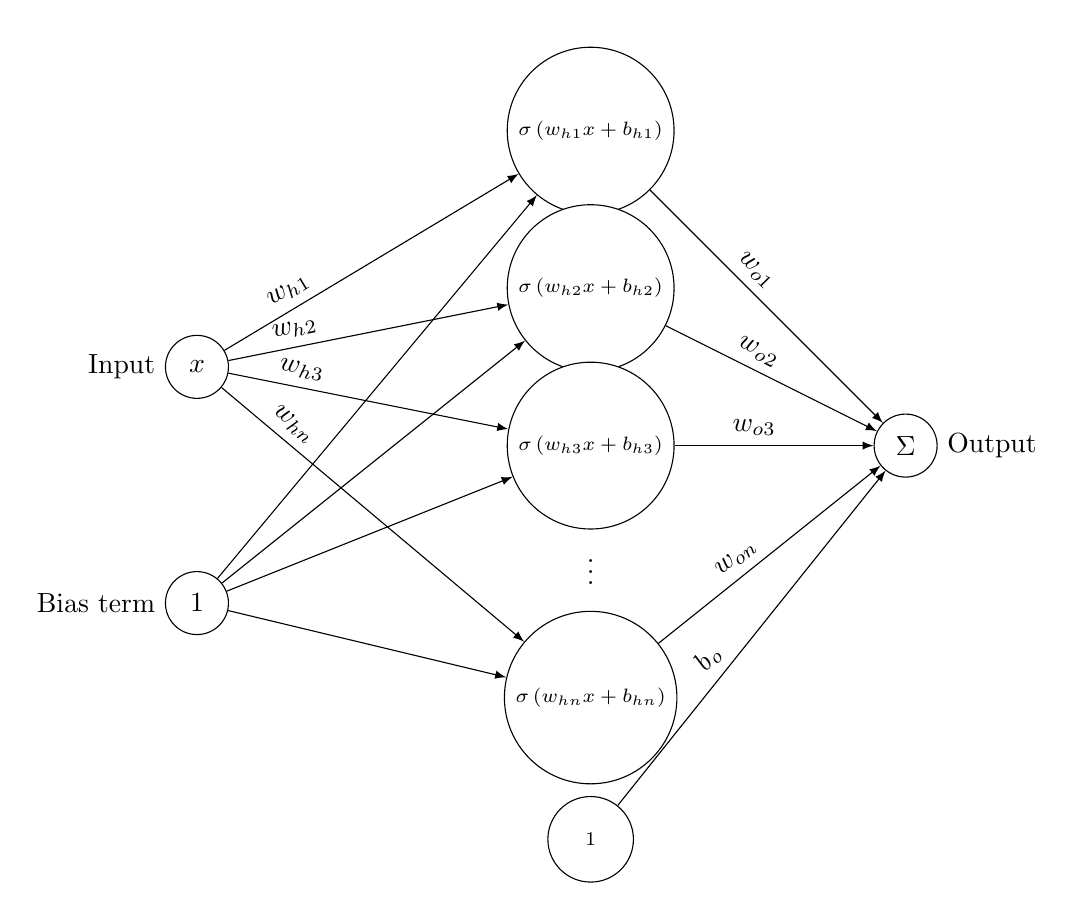
\begin{tikzpicture}
	[   cnode/.style={draw=black,draw=black,fill=#1,minimum width=8mm,circle},
	]
	\tikzset{normal arrow/.style={draw,-latex}}
	\node[cnode=white,label=0:Output] (s) at (9,-6) {$\Sigma$};
	\node[cnode=white,label=180:Bias term] (x-2) at (0,-8) {1};
	\node[cnode=white,label=180:] (p-5) at (5,-11) {1};
	\node at (5,-7.5) {$\vdots$};
	
	\node[cnode=white,label=180:Input] (x-1) at (0,-5) {$x$};
	
	\foreach \x in {1,...,5}
	{
		\pgfmathparse{\x<4 ? \x : "n"}	   
		\ifnum \x = 4
		
		
		\node[cnode=white,label=90:] (p-\x) at (5,{-2.05*\x-div(\x,4)}) {\scriptsize$\sigma\left(w_{hn}x + b_{hn}\right)$};
		
		\else
		
		\ifnum \x = 5
		
		
		\node[cnode=white,label=90:] (p-\x) at (5,{-2*\x-div(\x,4)}) {\scriptsize$\;\;\; \; 1 \; \;\;\;$};
		
		\else
		
		\node[cnode=white,label=90:] (p-\x) at (5,{-2*\x-div(\x,4)}) {\scriptsize$\sigma\left(w_{h\x}x + b_{h\x}\right)$};
		
		\fi
		
		
		\fi
		\ifnum \x = 5
		\path[normal arrow] (p-\x) -- node[above,sloped,pos=0.4] {$b_{o}$} (s);
		\else
		\path[normal arrow] (p-\x) -- node[above,sloped,pos=0.4] {$w_{o\pgfmathresult}$} (s);
		\fi
	}
	
	
	\foreach \x in {1,...,2}
	{   
		\foreach \y in {1,...,4}
		{   
			\ifnum \x=1
			\ifnum \y=4
			\path[normal arrow] (x-\x) -- (p-\y) node[above,sloped,pos=0.2] {$w_{h n}$};
			
			
			\else
			\ifnum \y=5
			\path[normal arrow] (x-\x) -- (p-\y) node[below,sloped,pos=0.15] {$w_{w n+1}$};
			\else 
			\path[normal arrow] (x-\x) -- (p-\y) node[above,sloped,pos=0.25] {$w_{h\y}$};
			
			\fi
			\fi
			\else
			\path[normal arrow] (x-\x) -- (p-\y); 
			
			\fi
			
			%\draw (x-\x) -- (p-\y) node[above,sloped,pos=0.3] {$\omega_{\x\y}$};
		}
	}
	\end{tikzpicture}
	
\end{center}



\def\layersep{2.5cm}
\begin{center}
	
	
	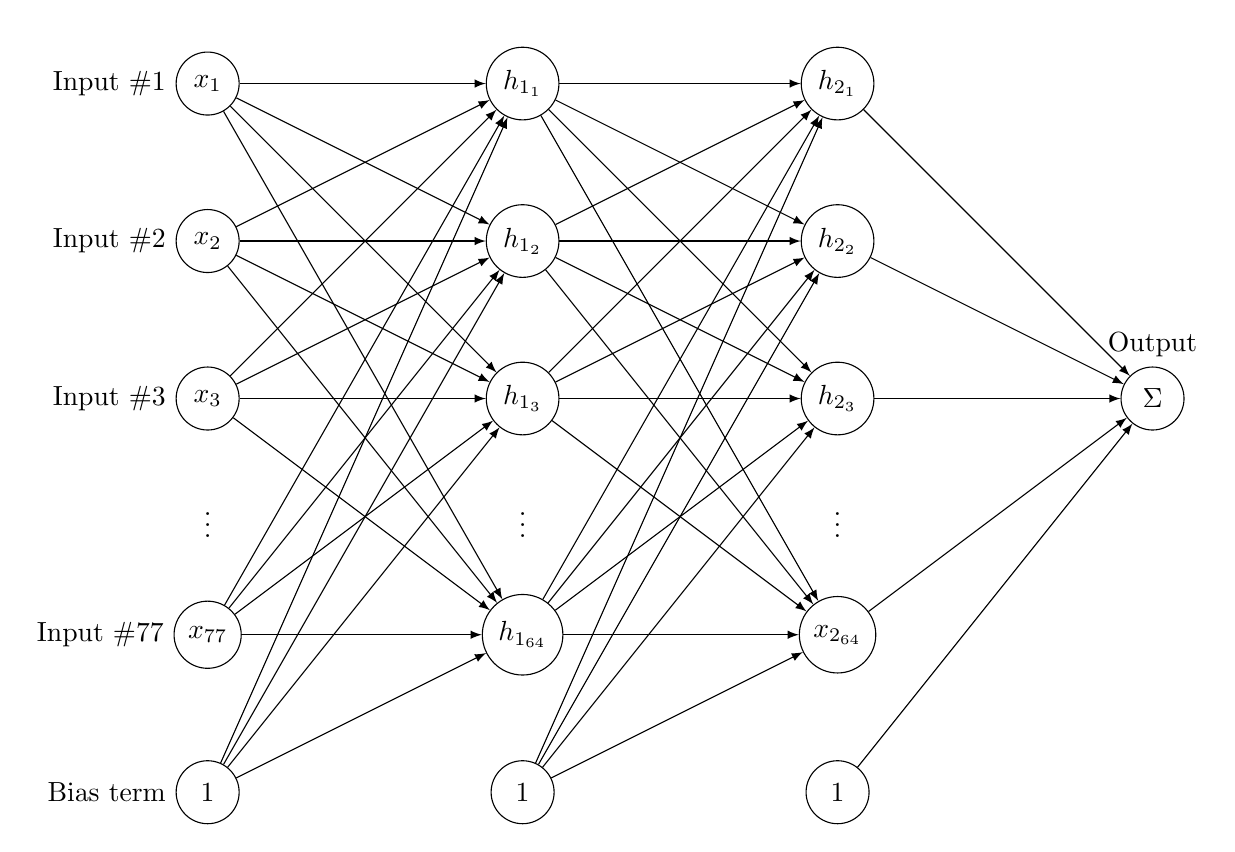
\begin{tikzpicture}
	[   cnode/.style={draw=black,draw=black,fill=#1,minimum width=8mm,circle},
	]
	\tikzset{normal arrow/.style={draw,-latex}}
	\node[cnode=white,label=90:Output] (s) at (12,-6) {$\Sigma$};
	\node at (0,-7.5) {$\vdots$};
	
	\node[cnode=white,label=180:Bias term] (x-5) at (0,-11) {1};
	
	\node at (4,-7.5) {$\vdots$};
	
	\node at (8,-7.5) {$\vdots$};
	
	\node[cnode=white,label=180:] (p-5) at (4,-11) {$1$};
	
	\node[cnode=white,label=180:] (z-5) at (8,-11) {$1$};
	
	
	\foreach \x in {1,...,4}
	{
		\pgfmathparse{\x<4 ? \x : "n"}	   
		\ifnum \x = 4
		\node[cnode=white,label=180:Input \#77] (x-\x) at (0,{-2*\x-div(\x,4)}) {$x_{77}$};
		\node[cnode=white,label=90:] (p-\x) at (4,{-2*\x-div(\x,4)}) {$h_{1_{64}}$};
		
		\node[cnode=white,label=90:] (z-\x) at (8,{-2*\x-div(\x,4)}) {$x_{2_{64}}$};
		
		\else
		
		\node[cnode=white,label=180:Input \#\pgfmathresult] (x-\x) at (0,{-2*\x-div(\x,4)}) {$x_{\x}$};
		\node[cnode=white,label=90:] (p-\x) at (4,{-2*\x-div(\x,4)}) {$h_{1_{\x}}$};
		
		\node[cnode=white,label=90:] (z-\x) at (8,{-2*\x-div(\x,4)}) {$h_{2_{\x}}$};
		
		\fi
		\path[normal arrow] (z-\x) -- node[above,sloped,pos=0.4] {} (s);
	}
	
	
	\foreach \x in {1,...,5}
	{   
		\foreach \y in {1,...,4}
		{   
			\ifnum \x=1
			\ifnum \y=4
			\path[normal arrow] (x-\x) -- (p-\y) node[above,sloped,pos=0.15] {};
			
			\else
			\path[normal arrow] (x-\x) -- (p-\y) node[above,sloped,pos=0.2] {};
			\fi
			\else
			\path[normal arrow] (x-\x) -- (p-\y); 
			
			\fi
			
			
			\ifnum \x=1
			\ifnum \y=4
			\path[normal arrow] (p-\x) -- (z-\y) node[above,sloped,pos=0.15] {};
			
			\else
			\path[normal arrow] (p-\x) -- (z-\y) node[above,sloped,pos=0.2] {};
			\fi
			\else
			\path[normal arrow] (p-\x) -- (z-\y); 
			
			\fi
			
			
			
			%\draw (x-\x) -- (p-\y) node[above,sloped,pos=0.3] {$\omega_{\x\y}$};
		}
		
		
		
		\ifnum \x=5
		\path[normal arrow] (z-\x) -- node[above,sloped,pos=0.4] {} (s);
		\else
		
		\fi
	}
	\end{tikzpicture}
	
\end{center}

